\documentclass[10pt]{amsart}
\usepackage[a4paper,margin=22mm]{geometry}
\usepackage[no-math]{fontspec}
\setmainfont{Latin Modern Roman}[SmallCapsFont={lmromancaps10-regular.otf}]
\usepackage{amsmath,amssymb,amsthm,mathtools,hyperref,graphicx,float}
\usepackage[shortlabels]{enumitem}
\emergencystretch=3em
\newtheorem{theo}{Theorem}[section]
\newtheorem{lemm}[theo]{Lemma}
\newtheorem{prop}[theo]{Proposition}
\newtheorem{coro}[theo]{Corollary}
\theoremstyle{definition}
\newtheorem{defi}[theo]{Definition}
\newtheorem{rema}[theo]{Remark}
\providecommand{\ie}{i.e.\ }
\DeclareMathOperator{\sgn}{sgn}
\DeclareMathOperator{\Tube}{Tube}
\DeclareMathOperator{\corr}{corr}
\DeclareMathOperator{\Vol}{Vol}
\DeclareMathOperator{\wt}{wt}
\DeclareMathOperator{\diag}{diag}

\newcommand{\RR}{\mathbb{R}}
\newcommand{\cJ}{\mathcal{J}}

\graphicspath{{./figures/}}

\newcommand*{\mk}{\mkern -1mu}
\newcommand*{\Mk}{\mkern -2mu}
\newcommand*{\mK}{\mkern 1mu}
\newcommand*{\MK}{\mkern 2mu}

\hypersetup{urlcolor=purple, linkcolor=blue, citecolor=red}

\newcommand*{\romanenumi}{\renewcommand*{\theenumi}{\roman{enumi}}}
\newcommand*{\Romanenumi}{\renewcommand*{\theenumi}{\Roman{enumi}}}
\newcommand*{\alphenumi}{\renewcommand*{\theenumi}{\alph{enumi}}}
\newcommand*{\Alphenumi}{\renewcommand*{\theenumi}{\Alph{enumi}}}
\title[Gaussian DAG partial-correlation nonsingularity]{Real nonsingularity of Gaussian DAG partial-correlation hypersurfaces under parent-to-conditioned-descendant adjacency}
\author{Jan Draisma}
\date{Algebraic Combinatorics2(3)(2019),439–446; DOI10.5802/alco.44}
\hypersetup{hidelinks}
% Resolve the three literal extensionless native graphic names to declared PDFs.
\let\originalBareGraphic\includegraphics
\renewcommand{\includegraphics}[2][]{\originalBareGraphic[#1]{#2.pdf}}
\begin{document}
\maketitle
\section{Introduction} \label{sec:Introduction}

\subsection*{DAGs}

Let $G$ be a directed, acyclic graph (DAG) with vertex set $V$ and edge set $D \subseteq \{(i,j) \in V^2 \mid i \neq j\}$. We write $i \to j$ if $(i,j) \in D$ and $i \not \to j$ otherwise. A path in $G$ from $i$ to $j$ of length $k$ is a sequence $(i=i_0,i_1,\ldots,i_k=j)$ with $i_{l} \to i_{l+1}$ for all $l=0,\ldots,k-1$; we allow $k=0$. If there exists a path from $i$ to $j$ of length at least $1$ we say that $j$ is below $i$.

\subsection*{Directed Gaussian graphical models}

We follow~\cite[p.~87]{Drton09}. Associated to $G$ is the directed graphical model for jointly Gaussian random variables $X_i,\ i \in V$ related~by
\[
X_j=\sum_{i: i \to j} a_{ij} X_i + \epsilon_j
\]
where the vector $\epsilon \sim \mathcal{N}(0,I)$ and where the $a_{ij} \in \RR$ are the parameters of the model. The vector $X=(X_j)_{j \in V}$ satisfies
\[
(I-A)^T X=\epsilon
\]
where $A$ is the matrix with $(i,j)$-entry $a_{ij}$ if $i
\to j$ and $0$ otherwise. Therefore $X\sim \mathcal{N}(0,\Sigma)$ where
\[
\Sigma=\Sigma(A)=(I-A)^{-T} (I-A)^{-1}.
\]
Note that, since $A$ is nilpotent, this is a matrix whose entries are polynomials in the parameters $a_{ij}, i \to j$. For subsets $I,J \subseteq V$ we write $\Sigma[I,J]$ for $I \times J$-submatrix $(\sigma_{ij})_{i \in I,j \in J}$ of $\Sigma$, and we use notation such as $I+i_0-s:=I \cup \{i_0\} \setminus \{s\}$.


\subsection*{Partial correlation hypersurfaces}

Let $i_0,j_0 \in V$ be distinct and $S \subseteq V \setminus \{i_0,j_0\}$. In~\cite{Uhler14} the \emph{partial correlation hypersurface} $H_f \subseteq \RR^D$ is defined as the zero locus of the polynomial
\[
f:=\det(\Sigma[S+i_0,S+j_0]);
\]
the expression $\corr(i_0,j_0|S):=f/\sqrt{\det(\Sigma[S+i_0,S+i_0])
\det(\Sigma[S+j_0,S+j_0])}$ is the partial correlation of $i_0$ and $j_0$ given $S$.

So the vanishing of $f$ is equivalent to the statement that $i_0,j_0$ are conditionally independent given $S$. We assume that $f$ is not identically zero on $\RR^D$. This is equivalent to the statement that $S$ does not \emph{d-separate} $i_0$ and $j_0$ in $G$~\cite[Section~2.3.4]{Spirtes01}; the trek system expansion of Section~\ref{sec:Background} yields an equivalent combinatorial characterisation.
\subsection*{Main result}

We will establish the following criterion for nonsingularity of $H_f$; the same applies when the $\epsilon_i$ have unequal variances (Proposition~\ref{prop:unequal}).

\begin{theo}
Assume that $i_0 \to j_0$ and that for all $s \in S$ below $j_0$ we have $i_0 \to s$. Then $H_f$ is nonsingular.
\end{theo}
\begin{coro}
If $G$ is the DAG on $\{1,\ldots,n\}$ with $i \to j$ if and only if $i<j$, then $H_f$ is nonsingular, independently of the choice of $i_0,j_0,S$.
\end{coro}

For $n \leq 6$ this is~\cite[Theorem~4.1]{Uhler14}, which was established there by extensive computer calculations showing that some power of $\det \Sigma[S+i_0+j_0,S+i_0+j_0]$ lies in the ideal generated by $f$ and its partial derivatives. Since $\Sigma[S+i_0+j_0,S+i_0+j_0]$ is positive definite and hence has a nonzero determinant for all (real) values of the parameters, this shows that the (real) common vanishing locus of $f$ and its derivatives is empty.

We will follow a similar approach, except that we consider the principal submatrix $\det \Sigma[S+i_0,S+i_0]$, no power is needed, and indeed not $f$ but only some of its partial derivatives are needed.
\section{Background} \label{sec:Background}

\subsection*{The trek rule}

We recall results from~\cite{Draisma09d}. Suppose we allow the variances of the $\epsilon_i$ to be distinct, rather than all equal to $1$ as above. In that case, the covariance matrix $\Sigma$ becomes
\[
\Sigma=(I-A)^{-T} \Omega (I-A)^{-1}
\]
where $\Omega$ is the diagonal matrix with the covariances of the $\epsilon_i$ on the diagonal. Using the geometric series for $(I-A)^{-1}$ we find that
\[
\sigma_{ij}=\sum_{t:i \to j} w(t)
\]
where the sum is over all \emph{treks} from $i$ to $j$ as in the following definition.

\begin{defi}
A \emph{trek} $t$ in $G$ is a pair $(P_U,P_D)$ of paths in $G$ that start at the same vertex $m$, the \emph{top} of the trek. The paths $P_U,P_D$ are called the \emph{up part} and the \emph{down part} of $t$, respectively. If $i_0$ is the last vertex of $P_U$ and $j_0$ is the last vertex of $P_D$, then we call $t$ is a trek \emph{from $i_0$ to $j_0$}, $i_0$ the \emph{starting} vertex of $t$, and $j_0$ the \emph{end} vertex of $t$. The \emph{weight} of $t$ equals
\[
w(t):= \left(\prod_{(i,j) \text{ in } P_U} a_{ij} \right) \cdot \omega_m \cdot
\left(\prod_{(i,j) \text{ in } P_D} a_{ij} \right).
\]
We allow one or both of $P_U,P_D$ to have length $0$, in which case the corresponding factor(s) above is (are) $1$.
\end{defi}

The terminology derives from an informal interpretation of a trek as traversing $P_U$ upwards from $i_0$ (\ie against the direction of its edges in $G$) and then traversing $P_D$ downwards to $j_0$. In slightly different terms, the \emph{trek rule} above goes back at least to~\cite{Wright34}.

\subsection*{Trek system expansion}

Equip $V$ with an arbitrary linear order. Then for $I,J \subseteq V$ of equal cardinality and $\pi:I \to J$ we define $\sgn(\pi)$ as $(-1)$ to the power the number of \emph{crossings}: pairs $(i_1,i_2) \in I^2$ with $i_1<i_2$ but $\pi(i_1)>\pi(i_2)$.

\begin{defi}
Let $I,J \subseteq V$ with $|I|=|J|=k$. A \emph{trek system} $T$ from $I$ to $J$ is a set of treks $\{t_1,\ldots,t_k\}$ such that $I$ is precisely the set of starting vertices of the $t_l$ and $J$ is precisely the set of end vertices of the $t_l$. We write $T:I \to J$. The map $\pi:I \to J$ that sends the starting vertex of each trek to its end vertex is a bijection, and we define the sign of $T$ as $\sgn(T):=\sgn(\pi)$. The weight of $T$ is $w(T):=\prod_{l=1}^k w(t_l)$.
\end{defi}

\begin{defi}
A \emph{sided intersection} between treks $t$ and $t'$ is a vertex where either the up parts of $t$ and $t'$ meet or the down parts of $t$ and $t'$ meet. We say that a trek system has no sided intersections if there is no sided intersection between any two of its treks.
\end{defi}

We have the following formula for subdeterminants of $\Sigma$.

\begin{prop}[\cite{Draisma09d}]
For $I,J \subseteq V$ of the same cardinality we have
\begin{equation}
\det \Sigma[I,J]=\sum_{T:I \to J \text{ without sided
intersections}} \sgn(T) \wt(T). \label{eq:nosided}
\tag{$\ast$}
\end{equation}
\end{prop}

The proof is an application of tail swapping as in the classical Lindstr\"om--Gessel--Viennot Lemma~\cite{Gessel85}. We will see another instance of tail swapping in Section~\ref{sec:Proof}. In~\cite{Draisma09d} the proposition is used to give a combinatorial criterion, generalising d-sepa\-ra\-tion, for the determinant to be identically zero on $\RR^D \times \RR_{>0}^V$. Furthermore, in~\cite{Draisma12h} it is shown that the sum above is cancellation-free: if two trek systems $I \to J$ have the same weight, then they have the same sign. Moreover, it is shown there that the coefficient of each monomial is plus or minus a power of $2$.

All of these results---the formula~\eqref{eq:nosided} of course, but also the cancellation-freeness and the power-of-two phenomenon---persist when we specialise $\Omega$ to the identity matrix, as we did in Section~\ref{sec:Introduction} and as we do again in Section~\ref{sec:Proof}. Indeed, if $T: I \to J$ is a trek system without sided intersection, then the tops of the treks in $T$ can be recovered from the specialisation of $w(T)$ as follows: $m$ is a top if and only if either
\begin{enumerate}
\item at least one $a_{mj}$ appears in $w(T)$ and no $a_{im}$ appears in $w(T)$; or else
\item $m \in I \cap J$ and $w(T)$ contains no $a_{mj}$ and no $a_{im}$ (then some trek is $((m),(m))$).
\end{enumerate}

\subsection*{Action by diagonal matrices}

Let $d=\diag((d_i)_{i \in V})$ where the $d_i$ are in $\RR_{>0}$. Then
\[
d \Sigma d= (d(I-A)^{-T}d^{-1}) \cdot (d \Omega d) \cdot (d^{-1}(I-A)^{-1}d)= (I-A')^{-T} \Omega' (I-A')^{-1}
\]
where $\Omega'=d \Omega d$ and where $A'=d^{-1}Ad$ has the same zero pattern as $A$. Hence, the group $(\RR_{>0})^V$ acts on the parameter space $\RR^D \times \RR_{>0}^V$ and on the space of covariance matrices in such a manner that the map $(a,\omega) \mapsto \Sigma$ is equivariant. This implies that for any $I, J \subseteq V$ of equal cardinality the hypersurface in $\RR^D \times \RR_{>0}^V$ defined by $\det \Sigma[I,J]=0$ is stable under this action.

Alternatively, this can be read off from~\eqref{eq:nosided}: scaling each $a_{ij}$ with $d_i^{-1} d_j$ and $\omega_m$ with $d_m^2$, the weight of each trek from a vertex $i \in I$ to a vertex $j \in J$ gets scaled by $d_i d_j$, and therefore $\det \Sigma[I,J]$ scales with $\big(\prod_{i \in I} d_i \big) \cdot \big(\prod_{j \in J} d_j\big)$.

Define $f_{\Omega}:=\det \Sigma[I,J]$ and let $f$ be obtained from $f_{\Omega}$ by specialising $\Omega$ to the identity matrix. Let $H_f$ be the hypersurface in $\RR^D$ defined by $f$ and let $H_{f_\Omega}$ be the hypersurface defined by $f_\Omega$ in $\RR^D \times \RR_{>0}^V$.

\begin{prop}\label{prop:unequal}
As semi-algebraic sets, $H_{f_\Omega}$ is isomorphic to $H_f \times
\RR_{>0}^V$. In particular, $H_{f_\Omega}$ is nonsingular if and only if $H_f$ is.
\end{prop}

\begin{proof}
By the discussion above, the map
\[
(a,d) \mapsto \left(\left(a_{ij} \cdot \frac{d_j}{d_i}\right)_{i \to j}, (d_m^2)_m\right)
\]
maps $H_f \times \RR_{>0}^V$ into $H_{f_\Omega}$. The inverse is given by
\[
(a',\omega) \mapsto \left(\left(a'_{ij} \cdot \frac{\sqrt{\omega_i}}{\sqrt{\omega_j}}\right)_{i \to j}, (\sqrt{\omega_m})_m \right).
\]
Both maps are morphisms of semi-algebraic sets.
\end{proof}


\section{Proof of the theorem} \label{sec:Proof}

We retain the notation of Section~\ref{sec:Introduction}; in particular, $\epsilon \sim \mathcal{N}(0,I)$, $f=\det \Sigma[S+i_0,S+j_0]$ and $H_f
\subseteq \RR^D$ is the hypersurface defined by $f$. In this section, we treat the $a_{ij}$ as variables and our computations take place in the polynomial ring $\RR[a_{ij} \mid (i,j) \in D]$. Let $\cJ$ be the ideal in this ring generated by all partial derivatives $\partial f/\partial a_{ij}$ of $f$.

\begin{lemm}\label{lm:sj}
For $s \in S$ and $j \in V$ with $s \to j$ the variable $a_{sj}$ does not appear in $f$.
\end{lemm}

\begin{proof}
Let $T:S+i_0 \to S+j_0$ be a trek system without sided intersection. If the arrow $s \to j$ were used in the up (respectively, down) part of some trek $t$ in $T$, then $t$ would have a sided intersection with the trek starting (respectively, ending) at $s$. So that arrow is not used and the conclusion follows from~\eqref{eq:nosided}.
\end{proof}

As a consequence, in the remaining discussion we may and will replace $D$ by $D \setminus S \times V$, so that \emph{$G$ has no arrows going out of $S$}.

\begin{lemm}\label{lm:i0s}
Suppose that $G$ has no outgoing arrows from elements of $S$. For $s \in S$ with $i_0 \to s$ the variable $a_{i_0s}$ appears at most linearly in $f$ and its coefficient equals $\pm \det
\Sigma[S+i_0,S+j_0-s+i_0]$. In particular, $\det \Sigma[S+i_0,S+j_0-s+i_0]
\in \cJ$.
\end{lemm}

\begin{proof}
If a trek $t$ in a trek system $T:S+i_0 \to S+j_0$ without sided intersection uses the edge $i_0 \to s$, then it does so in its down part---indeed, in its up part it would yield a sided intersection with the trek starting at $i_0$. In particular, the variable $a_{i_0s}$ appears only linearly in $f$. Furthermore, $t$ ends in $s$, or else $t$ would have a sided intersection with the trek ending at $s$.

So if we remove from $t$ the arrow $i_0
\to s$, then we obtain a trek system $T':S+i_0 \to S+j_0-s+i_0$ without sided intersection~(Figure~\ref{fig:i0s}).

\begin{figure}
\begin{center}
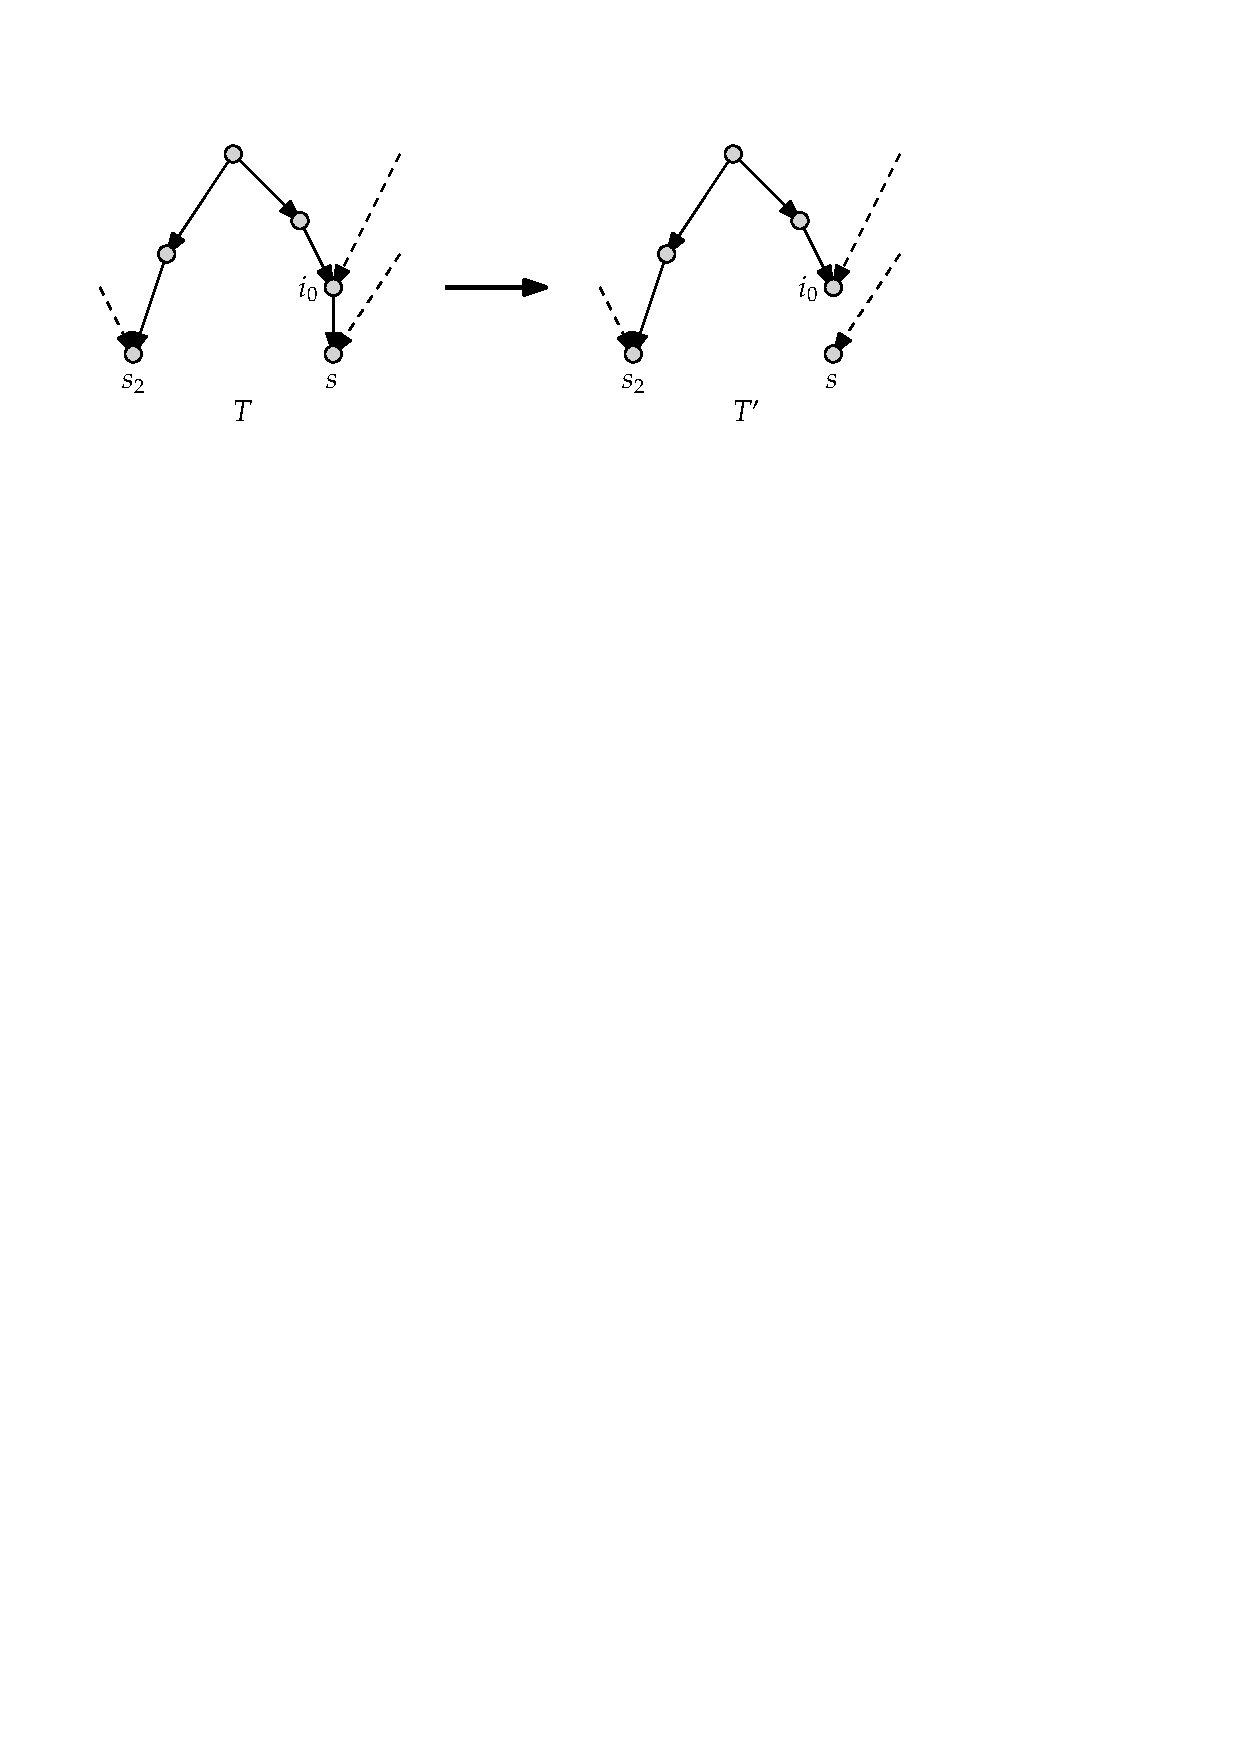
\includegraphics[scale=.7]{1664-assets/i0s}
\end{center}
\caption{Proof of Lemma~\ref{lm:i0s}. We suggestively draw the arrows in up parts of treks as pointing in the south-west direction and arrows in down parts as pointing in the south-east direction---of course, this is not always possible!}\label{fig:i0s}
\end{figure}

Conversely, if we have any trek system $T':S+i_0 \to S+j_0-s+i_0$ without sided intersection, then no trek in it passes through $s$ on its way down, because $s$ has no outgoing arrows. Hence, adding the arrow $i_0 \to s$ to the trek $t'$ in $T'$ ending in $i_0$ yields a trek system $S+i_0
\to S+j_0$ without sided intersection.

Hence the map $T \mapsto T'$ gives a bijection between the terms in (the trek system expansion of) $f$ divisible by $a_{i_0s}$ and the terms in $\det \Sigma[S+i_0,S+j_0+i_0-s]$. Furthermore, $\sgn(T)$ equals $\pm
\sgn(T')$, where the sign is the sign of the bijection $S+j_0-s+i_0
\to S+j_0$ that is the identity on $S+j_0-s$ and sends $i_0$ to $s$; in particular, this sign does not depend on $T$.
\end{proof}

\begin{lemm}\label{lm:i0j0}
Assume that $i_0 \to j_0$. The variable $a_{i_0j_0}$ appears at most linearly in $f$ and its coefficient equals $\pm(\det \Sigma[S+i_0,S+i_0]-g)$ where
\begin{equation}\label{eq:i0j0}
g=\sum_{T'':S+i_0 \to S+i_0} \sgn(T'') w(T'')
\tag{$\ast\ast$}
\end{equation}
is the sum over all trek systems $T'':S+i_0 \to S+i_0$ without sided intersection \emph{of which one trek contains $j_0$ in its down part}. In particular, $\det \Sigma[S+i_0,S+i_0] - g \in
\cJ$.
\end{lemm}

\begin{proof}
If a trek $t$ in a trek system $T:S+i_0 \to S+j_0$ without sided intersection uses the edge $i_0 \to j_0$, then it does so on its way down: on its way up it would yield a sided intersection with the trek starting at $i_0$. In particular, the variable $a_{i_0j_0}$ appears only linearly in $f$.

Furthermore, $t$ ends in $j_0$, or else it would have a sided intersection with the trek ending at $j_0$. So if we remove from $t$ the arrow $i_0
\to j_0$, then we obtain a trek system $T'':S+i_0 \to S+i_0$ without sided intersection~(Figure~\ref{fig:i0j0}). Also, $\sgn(T)$ equals $\sgn(T'')$ times the sign of the bijection $S+i_0 \to S+j_0$ that is the identity on $S$ and maps $i_0$ to $j_0$; this will determines the sign $\pm$ in the lemma.

\begin{figure}
\begin{center}
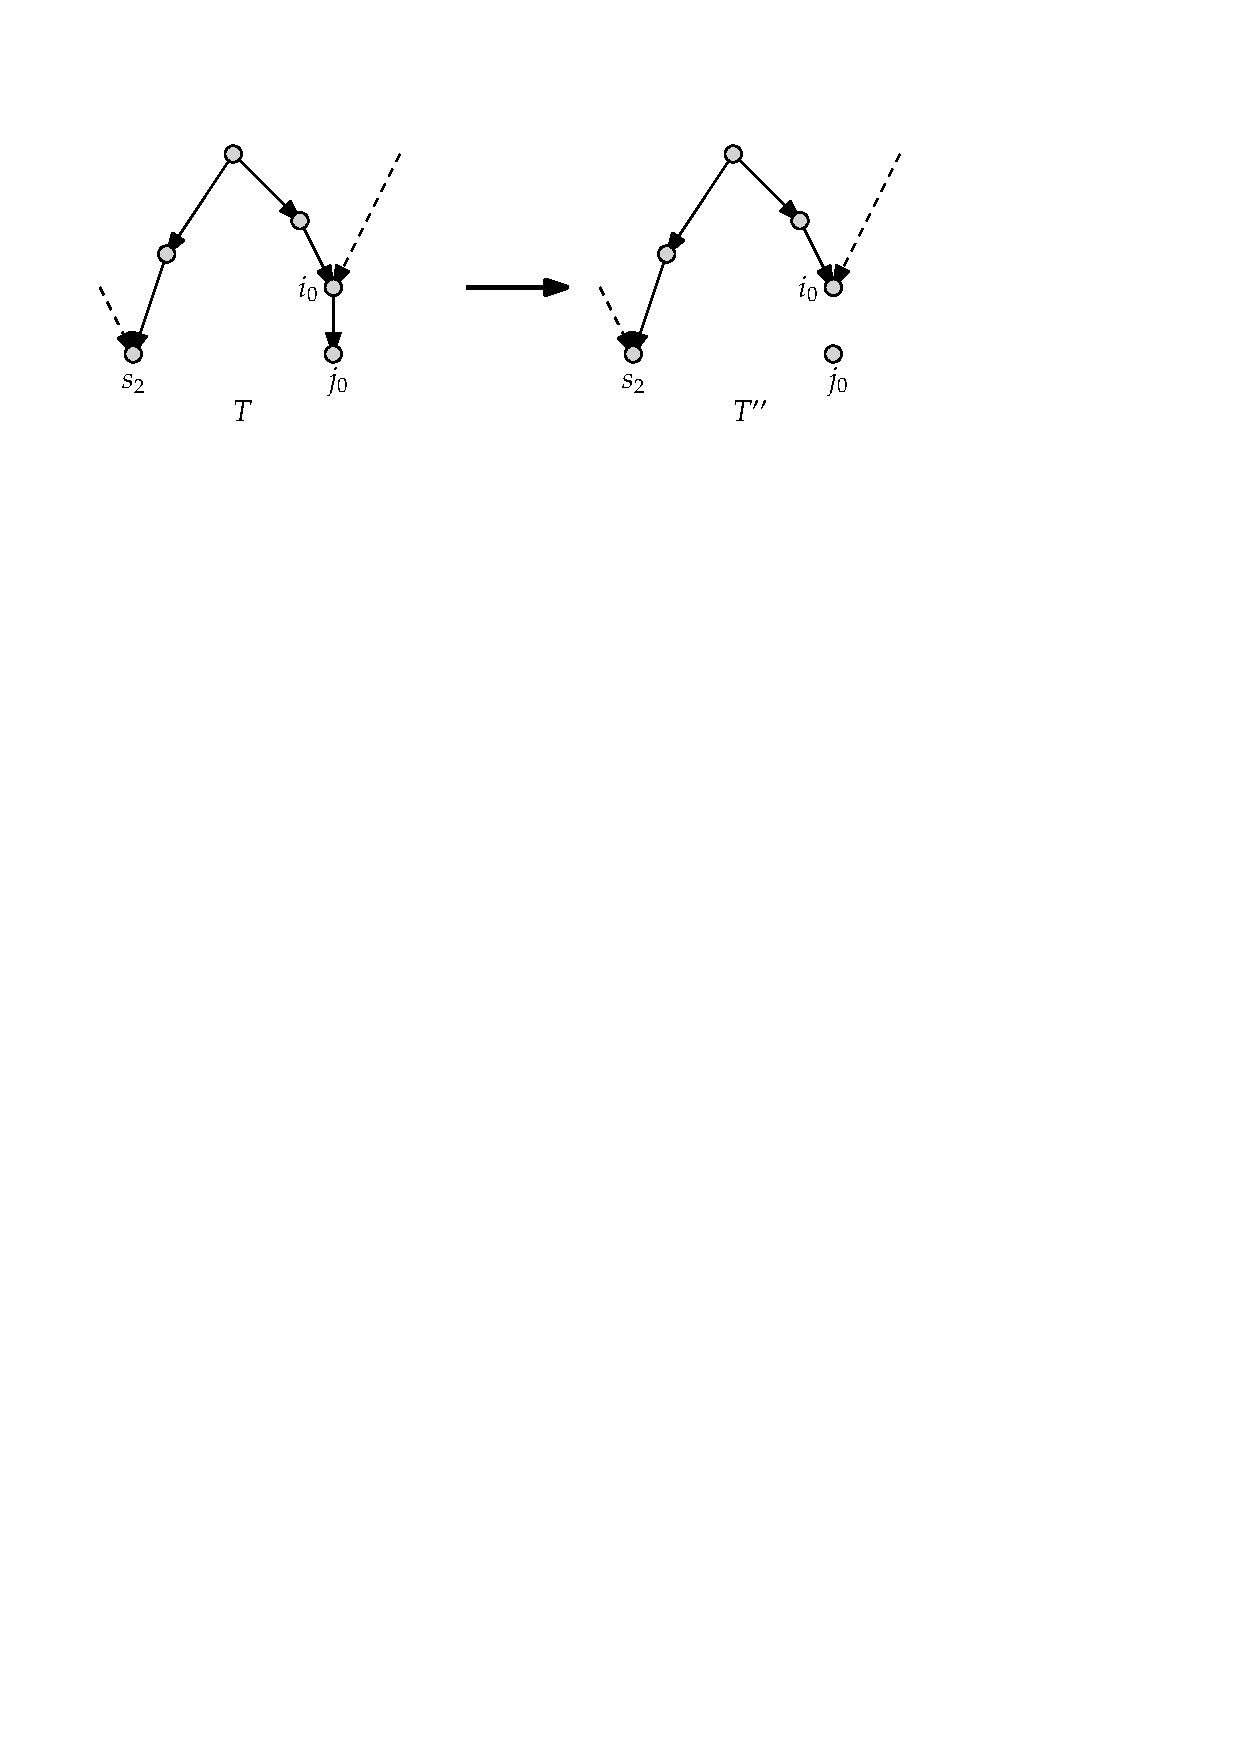
\includegraphics[scale=.7]{1664-assets/i0j0}
\end{center}
\caption{Proof of Lemma~\ref{lm:i0j0}.}\label{fig:i0j0}
\end{figure}

Conversely, given a trek system $T'':S+i_0 \to S+i_0$ without sided intersection, we may try and add the arrow $i_0 \to j_0$ to the trek ending in $i_0$. The resulting trek system has no sided intersection if and only if no trek of $T''$ passes $j_0$ on its way down. The remaining $T''$ must be therefore be subtracted as in the lemma.
\end{proof}

For $s \in S$ below $j_0$ define $p_{j_0,s}:=\sum_{P:j_0 \to s} w(P)$, the sum of the weights of all directed paths in $G$ from $j_0$ to $s$.

\begin{lemm}\label{lm:id}
The element $g$ from~\eqref{eq:i0j0} satisfies
\[
g=\sum_{s \in S \text{ under } j_0} \sgn(\pi_s) \det \Sigma[S+i_0,S+i_0-s+j_0]
\cdot p_{j_0,s}
\]
where $\pi_s:S+i_0-s+j_0 \to S+i_0$ is the identity on $S+i_0-s$ and sends $j_0$ to $s$.
\end{lemm}

\begin{proof}
Let $T':S+i_0 \to S+i_0-s+j_0$ be a trek system without sided intersection and let $t'$ be the trek of $T'$ ending in $j_0$. Appending to $t'$ any path from $j_0$ down to $s$ yields a trek system $T'':S+i_0 \to S+i_0$ with sign $\sgn(T'')=\sgn(T') \sgn(\pi_s)$. In this manner, precisely those trek systems $T'':S+i_0 \to S+i_0$ arise for which
\begin{enumerate}
\item \label{p3.4.1} a unique trek $t''$ of $T''$ passes $j_0$ on its way down, and
\item \label{p3.4.2} every sided intersection of $T''$ is between $t''$ and some other trek of $T''$ on their way down, and happens at a vertex below $j_0$.
\end{enumerate}
So the left-hand side of the equation in the lemma equals $\sum_{T'':S+i_0
\to S+i_0} \sgn(T'')\times w(T'')$ where $W''$ runs over the trek systems with properties~\eqref{p3.4.1} and~\eqref{p3.4.2}. The right-hand side is the sub-sum over all $T''$ without any sided intersection. We construct a sign-changing involution on the remaining $T''$, as follows.

Let $k$ be the \emph{lowest} vertex on the down part of $t''$ that lies on the down part of some other trek $u'' \neq t''$ of $T''$. Swapping the parts of $t''$ and $u''$ below $k$ yields treks $t'''$ and $u'''$ that still meet at $k$. Let $T'''$ be the trek system obtained from $T''$ by replacing $t''$ with $t'''$ and $u''$ with $u'''$ (Figure~\ref{fig:id}).

\begin{figure}
\begin{center}
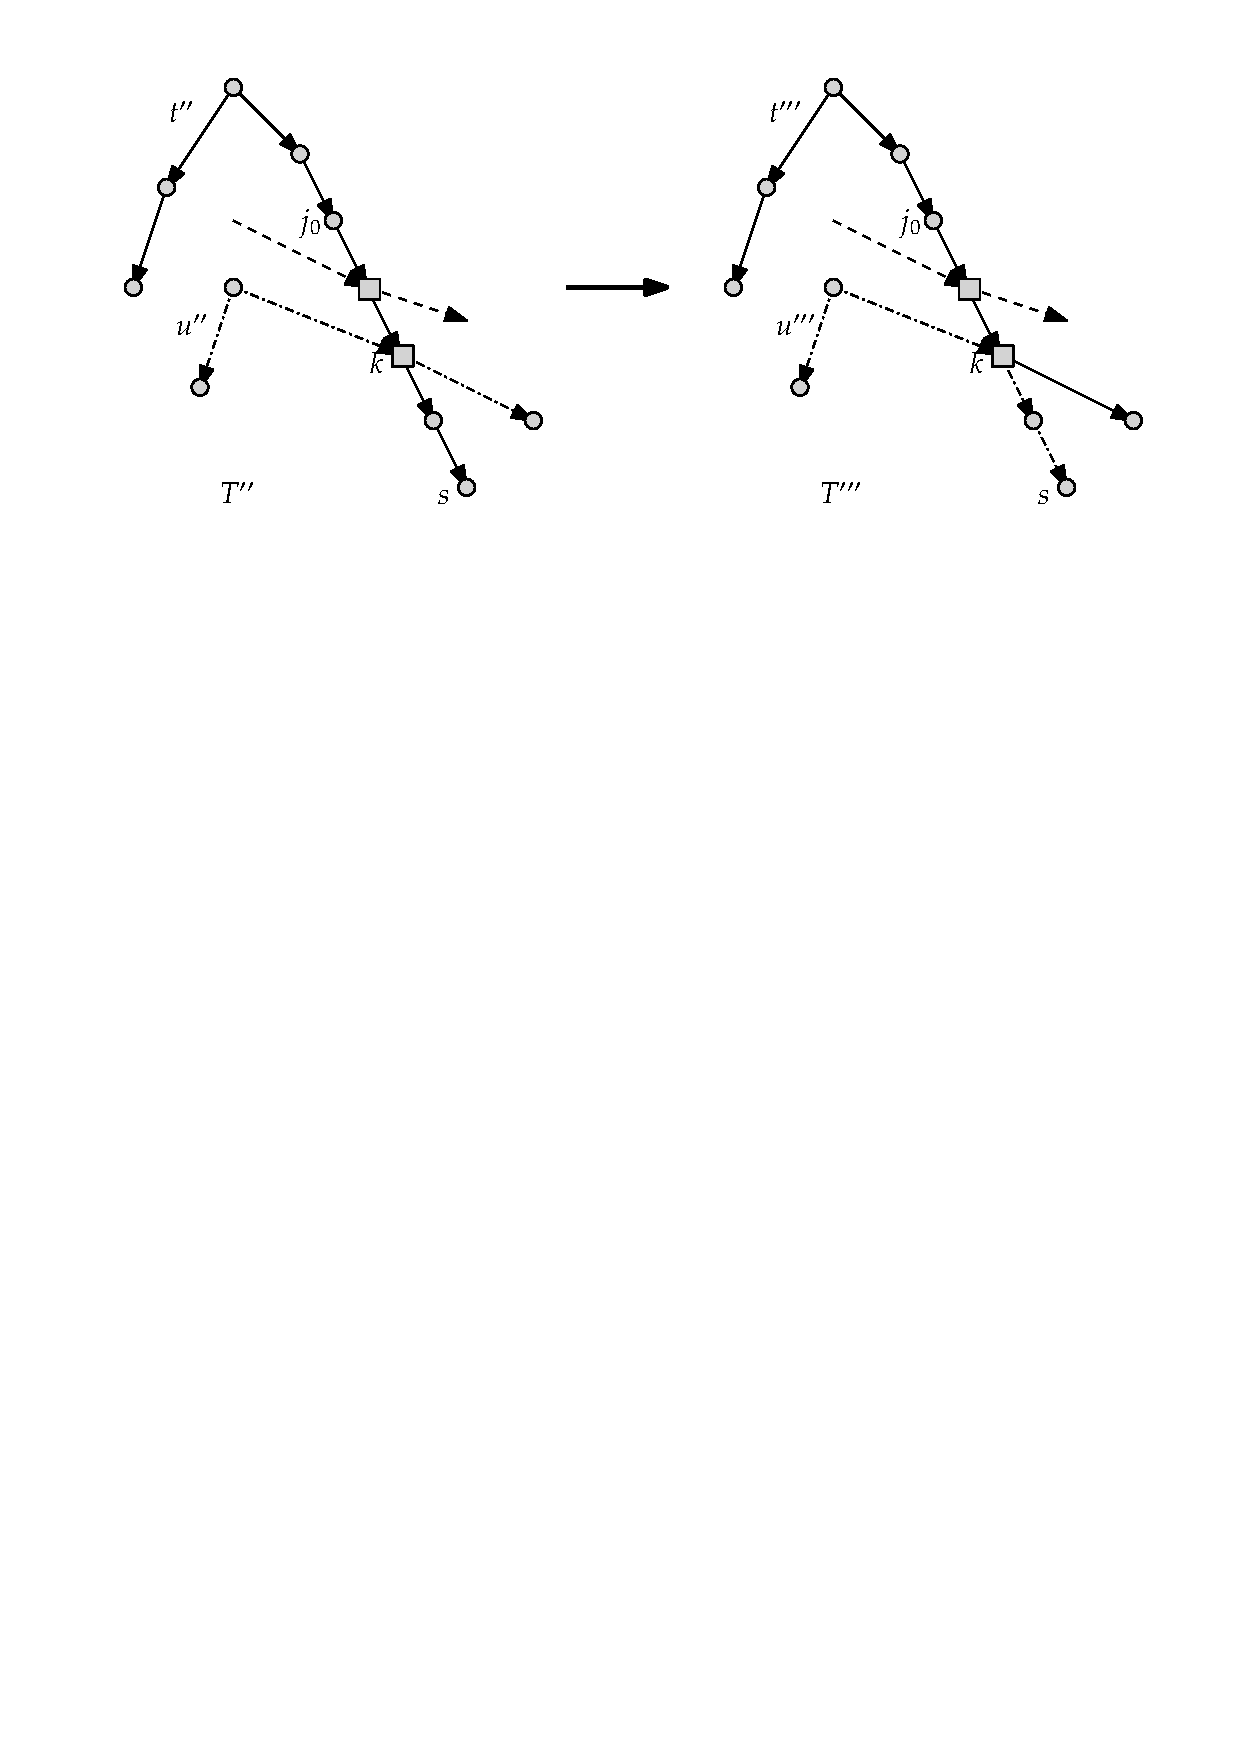
\includegraphics[scale=.7]{1664-assets/id}
\caption{The tail swapping argument of Lemma~\ref{lm:id}. The sided intersections of $t''$ with other treks are depicted as square vertices.}\label{fig:id}
\end{center}
\end{figure}

The trek system $T'''$ satisfies~\eqref{p3.4.1}: $t'''$ is its unique trek that passes $j_0$ on its way down. As for~\eqref{p3.4.2}: the sided intersections between $t'''$ and other treks are precisely the sided intersections between $t''$ and other treks, so they happen below $j_0$. Also, $u'''$ cannot have sided intersections with treks other than $t'''$, because those would have come from a sided intersection between $t'''$ and another trek happening below $k$---this is where the choice of $k$ matters. Furthermore, $T''' \setminus \{t''',u'''\}=T'' \setminus \{t'',u''\}$, so there are no sided intersections between these treks. This shows that $T'''$ satisfies~\eqref{p3.4.2}. Also, the map $T'' \to T'''$ is an involution, since $k$ is the last intersection of the down part of $t'''$ with any down part of a trek in $T'''$. Since $\sgn(T''')=-\sgn(T'')$, this shows that the terms on the left-hand side that do not appear in the right-hand side cancel out.
\end{proof}
\begin{proof}[Proof of the theorem]
We claim that the zero set of $\cJ$ in $\RR^D$ is empty. By Lemma~\ref{lm:sj} we may delete from $G$ all outgoing arrows from elements of $S$ without changing $f$. Since $i_0 \to j_0$, by Lemma~\ref{lm:i0j0} we have $\det \Sigma[S+i_0,S+i_0]-g \in \cJ$. The identity in Lemma~\ref{lm:id} expresses $g$ as a linear combination of the determinants in Lemma~\ref{lm:i0s} where $s$ runs over the elements of $S$ below $j_0$. By assumption, for each of these $s$ we have $i_0 \to s$, so Lemma~\ref{lm:i0s} implies that $g \in \cJ$. Hence $\det \Sigma[S+i_0,S+i_0]
\in \cJ$. But for any set of real parameters $a \in \RR^D$ the matrix $\Sigma[S+i_0,S+i_0]$ is positive definite, hence has a nonzero determinant. This proves the claim.
\end{proof}
\begin{thebibliography}{99}
\bibitem[1]{Draisma12h} Draisma, Jan; Sullivant, Seth; Talaska, Kelli Positivity for Gaussian graphical models, Adv. Appl. Math., Volume 50 (2013) no. 5, pp. 661-674.
\bibitem[2]{Drton09} Drton, Mathias; Sturmfels, Bernd; Sullivant, Seth Lectures on algebraic statistics, Oberwolfach Seminars, 39, Birkhäuser, 2009, viii+271 pages.
\bibitem[3]{Gessel85} Gessel, Ira; Viennot, Gérard Binomial determinants, paths, and hook length formulae, Adv. Math., Volume 58 (1985), pp. 300-321.
\bibitem[4]{Uhler14} Lin, Shaowei; Uhler, Caroline; Sturmfels, Bernd; Bühlmann, Peter Hypersurfaces and their singularities in partial correlation testing, Found. Comput. Math., Volume 14 (2014) no. 5, pp. 1079-1116.
\bibitem[5]{Spirtes01} Spirtes, Peter; Glymour, Clark; Scheines, Richard Causation, prediction, and search. With additional material by David Heckerman, Christopher Meek, Gregory F. Cooper and Thomas Richardson., MIT Press, 2001, xxii+496 pages.
\bibitem[6]{Draisma09d} Sullivant, Seth; Talaska, Kelli; Draisma, Jan Trek separation for Gaussian graphical models, Ann. Stat., Volume 38 (2010) no. 3, pp. 1665-1685.
\bibitem[7]{Wright34} Wright, Sewall The method of path coefficients, Ann. Math. Stat., Volume 5 (1934), pp. 161-215.
\end{thebibliography}
\end{document}
